%%%%%%%%%%%%%%%%%%%%%%%%%%%%%%%%%%%%%%%%%%%%%%%%%%%%%%%%%%%%%%%%%%%%%
% LaTeX Template: Project Titlepage Modified (v 0.1) by rcx
%
% Original Source: http://www.howtotex.com
% Date: February 2014
% 
% This is a title page template which be used for articles & reports.
% 
% This is the modified version of the original Latex template from
% aforementioned website.
% 
%%%%%%%%%%%%%%%%%%%%%%%%%%%%%%%%%%%%%%%%%%%%%%%%%%%%%%%%%%%%%%%%%%%%%%

\documentclass[12pt]{report}
\usepackage[a4paper]{geometry}
\usepackage[myheadings]{fullpage}
\usepackage{xcolor}
\definecolor{shiftlyblue}{HTML}{111344}
\definecolor{shiftlypurple}{HTML}{52154E}
\usepackage{fancyhdr}
\usepackage{lastpage}
\usepackage{graphicx, wrapfig, subcaption, setspace, booktabs}
\usepackage{float}
\usepackage[T1]{fontenc}
\usepackage[font=small, labelfont=bf]{caption}
\usepackage{fourier}
\usepackage[protrusion=true, expansion=true]{microtype}
\usepackage[english]{babel}
\usepackage{sectsty}
\usepackage{url, lipsum}
\usepackage{tgbonum}
\usepackage{hyperref}
\usepackage{xcolor}

\newcommand{\HRule}[1]{\rule{\linewidth}{#1}}
\onehalfspacing
\setcounter{tocdepth}{5}
\setcounter{secnumdepth}{5}



%-------------------------------------------------------------------------------
% HEADER & FOOTER
%-------------------------------------------------------------------------------
%\pagestyle{fancy}
%\fancyhf{}
%\setlength\headheight{15pt}
%\fancyhead[L]{Student ID: 1034511}
%\fancyhead[R]{Anglia Ruskin University}
%\fancyfoot[R]{Page \thepage\ of \pageref{LastPage}}
%-------------------------------------------------------------------------------
% TITLE PAGE
%-------------------------------------------------------------------------------

\begin{document}
{\fontfamily{cmr}\selectfont
\begin{titlepage}
\begin{center}
\vspace*{0.1cm}
\IfFileExists{upp.png}{

\includegraphics[width=0.16\textwidth]{upp.png}
\par\vspace{0.2cm}
}{}
{\Large
\textcolor{shiftlyblue}{\textbf{UNIVERSIDAD POLITÉCNICA DE PACHUCA}}
\par}
\vspace{0.20cm}
{\large
\textcolor{shiftlyblue}{\textbf{TECNOLOGÍAS DE LA INFORMACIÓN E INNOVACIÓN DIGITAL}}
\par}
\vspace{0.6cm}
\textcolor{shiftlypurple}{\rule{\textwidth}{1.2pt}}
\vspace{0.4cm}
{\Large
\textcolor{shiftlypurple}{\textbf{APLICACIONES WEB}}
\par}
\vspace{0.35cm}
{\LARGE
\textbf{SHIFTLY}
\par}
\vspace{0.2cm}
{\huge
\textcolor{shiftlypurple}{\textbf{REPORTE DEL PROYECTO}}
\par}
\vspace{0.4cm}
\textcolor{shiftlypurple}{\rule{\textwidth}{1.2pt}}
\vspace{0.1 cm}
{\large \textbf{Docente}}
\par
\vspace{0.1cm}
{\large Yeniza Sarahí Montoya Martínez}
\par
\vspace{0.1cm}
{\large \textbf{Integrantes del equipo}}
\par
\vspace{0.1cm}
{\normalsize
Luis David Balandrano Delgado\\
Keydhy Mareli Villa Aldana\\
Isis Dayane Arellano Carillo\\
Vaneza Lugo Ramirez\\
Brian Jael Juarez Rodriguez\\
Julio Cesar Licona Acosta\\
\par}
\vspace{0.7cm}
{\large
\textbf{GRUPO: 04\_02}
\par}
\vfill
{\normalsize
\textbf{Fecha:} 5 de octubre de 2026
\par}
\end{center}
\end{titlepage}
\tableofcontents
\newpage

%-------------------------------------------------------------------------------
% Section title formatting
\sectionfont{\scshape}
%-------------------------------------------------------------------------------

%-------------------------------------------------------------------------------
% BODY
%-------------------------------------------------------------------------------
% =====================================================
% DOCUMENTACIÓN DEL PROYECTO SHIFT
% =====================================================

\section{Introducción}
SHIFTLY es una aplicación web orientada al aprendizaje del idioma inglés,
diseñada para adaptar el contenido de aprendizaje de acuerdo con el nivel
y los intereses del usuario, la aplicación busca proporcionar una experiencia de aprendizaje organizada mediante diferentes áreas de contenido, lecciones, vocabulario, ejercicios interactivos y seguimiento del progreso, desta manera, el usuario puede
avanzar dentro de una ruta de aprendizaje de acuerdo a sus necesidades e
intereses el desarrollo del proyecto se realiza mediante tecnologías web y un proceso
de trabajo colaborativo, utilizando HTML, CSS, Bootstrap y herramientas decontrol de versiones como Git y GitHub
\subsection{Objetivo}
El objetivo de SHIFTLY es desarrollar una aplicacion web de aprendizaje de inglés
que permita al usuario realizar un diagnóstico inicial, seleccionar un área
de aprendizaje de interés, acceder posteriormente a contenidos y
actividades adaptadas a su proceso de aprendizaje. El proyecto busca integrar una experiencia de aprendizaje que incluya vocabulario, lecciones, ejercicios interactivos, evaluaciones y seguimiento del progreso del usuario.
\subsubsection{Alcance del Proyecto}
A corto plazo buscamos comprender el desarrollo inicial de la aplicación web ,terminar un prototipo funcional en donde se muetre registro y inicio de sesión del usuarios, edición de perfil de usuario, selección del nivel de inglés del usuario, selección del área de aprendizaje de interés ya sea programación, gastronomía, turismo, negocios o inglés cotidiano.
\\{El objetivo a mediano plazo sera convertir el prototipo inicial en una aplicación web funcional, incorporando las principales características para ofrecer una experiencia completa de aprendizaje como la visualización de módulos y lecciones de acuerdo con el nivel y área de aprendizaje seleccionados, incorporación de vocabulario especializado, traducciones, definiciones, ejemplos y material de apoyo, implementación de ejercicios interactivos para reforzar el aprendizaje.}
\\{A largo plazo el objetivo será continuar el desarrollo de SHIFTLY y convertirla en una aplicación con potencial comercial, posiblemente surga la incorporación de nuevas funcionalidades y la creación de un modelo de negocio que permita generar ingresos}



\section{Alcance del proyecto}
El proyecto SHIFTLY contempla el desarrollo de un prototipo de una
aplicación web orientada al aprendizaje del idioma inglés. La propuesta
busca ofrecer una experiencia de aprendizaje organizada y adaptable a los
intereses y necesidades del usuario. Como parte del alcance inicial, la aplicación contempla el registro e inicio de sesión del usuario, la realización de un diagnóstico para determinar su nivel de inglés y la selección de un área de aprendizaje.
Las áreas de aprendizaje consideradas son:
\begin{itemize}
\item Programación
\item Gastronomía
\item Turismo
\item Negocios
\item Inglés cotidiano
\end{itemize}
Después de seleccionar su área de interés, el usuario podrá acceder a
diferentes contenidos de aprendizaje, incluyendo lecciones, vocabulario y
ejercicios interactivos. También se contempla la evaluación de las
actividades y el seguimiento del progreso del usuario. El proyecto incluye diferentes interfaces que representan las principales funciones de la aplicación, entre ellas el diagnóstico inicial, la selección de áreas de aprendizaje, el dashboard, las tarjetas de
vocabulario, los ejercicios interactivos, el mapa de lecciones, la biblioteca y repaso, los resultados y las recomendaciones de aprendizaje.
El desarrollo corresponde a un prototipo inicial por lo tanto, algunas
funcionalidades se presentan principalmente a nivel visual y de
interacción de acuerdo con los objetivos establecidos para esta primer etapa del
proyecto

\section{Equipo de trabajo y responsabilidades}
\subsection{Integrantes del equipo}
El desarrollo de SHIFT se realizó mediante un equipo de trabajo organizado en diferentes roles y responsabilidades, cada integrante participó en una parte específica del desarrollo de la aplicación web, permitiendo distribuir las actividades de análisis, diseño y programación.
\begin{itemize}
\item \textbf{Luis David Balandrano Delgado -- Líder técnico:} encargado de coordinar el desarrollo técnico del proyecto, organizar las actividades del equipo y supervisar la integración de los diferentes componentes de la aplicación
\item \textbf{Keydhy Mareli Villa Aldana -- Analista:} encargada del análisis y documentación del proyecto, así como de la elaboración y organización de los requerimientos, documentación técnica y evidencias del desarrollo
\item \textbf{Isis Dayane Arellano Carillo -- Frontend:} encargada del desarrollo de interfaces relacionadas con el diagnóstico inicial y el dashboard principal del usuario
\item \textbf{Vaneza Lugo Ramírez -- Backend:} encargada del desarrollo de funcionalidades relacionadas con las tarjetas de vocabulario y la biblioteca o sección de repaso
\item \textbf{Brian Jael Juárez Rodríguez -- Frontend:} encargado del desarrollo de las interfaces correspondientes a los ejercicios interactivos de aprendizaje
\item \textbf{Julio  Cesar Licona Acosta -- Backend:} encargado del desarrollo de funcionalidades relacionadas con el mapa de lecciones y las recomendaciones de la siguiente lección
\end{itemize}

\subsection{Distribución de interfaces}
La distribución de las interfaces se realizó de acuerdo con las actividades asignadas a cada integrante mediante el sistema de Issues del repositorio de GitHub
\begin{itemize}
\item \textbf{Keydhy -- Selección de áreas de aprendizaje:} desarrolló la pantalla donde el usuario selecciona el área de inglés que desea aprender. La interfaz incluye las opciones de Programación, Gastronomía, Turismo, Negocios e Inglés cotidiano, además de la selección visual y la validación del botón de continuar.
\item \textbf{Isis -- Diagnóstico inicial:} desarrolló la pantalla del diagnóstico inicial, destinada a evaluar el nivel de inglés del usuario mediante preguntas, selección de respuestas y presentación del resultado final.
\item \textbf{Isis -- Dashboard y progreso:} desarrolló el dashboard principal del alumno, incluyendo elementos visuales para mostrar el progreso general, la racha de días y gráficas de avance.
\item \textbf{Brian -- Ejercicios interactivos:} desarrolló las vistas de ejercicios para practicar el idioma mediante actividades como completar frases, arrastrar palabras, selección múltiple y emparejamiento.
\item \textbf{Vaneza -- Tarjetas de vocabulario:} desarrolló las tarjetas de aprendizaje o flashcards, incluyendo la palabra en inglés, traducción, definición, pronunciación y ejemplos.
\item \textbf{Vaneza -- Biblioteca y repaso:} desarrolló la pantalla de repaso y glosario, con una organización visual del vocabulario aprendido y opciones de búsqueda y filtros.
\item \textbf{Julio -- Mapa de lecciones:} desarrolló la vista de árbol o ruta de aprendizaje, donde se representan las lecciones desbloqueadas, bloqueadas y completadas.
\item \textbf{Julio 
-- Recomendación de siguiente lección:} desarrolló la sección destinada a mostrar una recomendación de la siguiente lección dentro del dashboard.
\item \textbf{Luis David -- Autenticación:} desarrolló las interfaces relacionadas con el registro de usuario, inicio de sesión, recuperación de contraseña, verificación por correo y perfil.
\item \textbf{Luis David -- Resultados y calificación:} desarrolló la pantalla de finalización de la lección, donde se presenta la calificación, puntuación y resumen de aciertos y errores.
\end{itemize}


\section{Requerimientos específicos}
Los requerimientos específicos de SHIFTLY describen las funciones y
características que debe cumplir la aplicación web. Estos requerimientos se
dividen en requerimientos funcionales y requerimientos no funcionales, los requerimientos funcionales describen las acciones y servicios que la aplicación debe proporcionar al usuario, mientras que los requerimientos no funcionales establecen características relacionadas con la calidad, usabilidad, rendimiento, seguridad y funcionamiento del sistema.
    
    

\section{Requerimientos funcionales}
Los requerimientos funcionales describen las funciones principales que
realizará la aplicación web SHIFTLY, proporcionando al usuario una
experiencia adecuada de aprendizaje.
\subsubsection{RF-001 Registro de usuario}
La aplicación web deberá permitir al usuario crear una cuenta
proporcionando los datos solicitados para acceder a la aplicación y
guardar su progreso
\textbf{Prioridad: Alta}
\subsubsection{RF-002 Diagnóstico de nivel}
La aplicación web deberá permitir al usuario realizar una evaluación
inicial para determinar su nivel de conocimiento del idioma inglés
\textbf{Prioridad: Alta}
\subsubsection{RF-003 Selección de área de aprendizaje}
La aplicación web deberá permitir al usuario seleccionar un área de
aprendizaje entre las opciones disponibles, con el propósito de adaptar
el contenido a sus intereses
\textbf{Prioridad: Alta}
\subsubsection{RF-004 Lecciones por nivel}
La aplicación web deberá mostrar al usuario las lecciones correspondientes
al nivel de inglés obtenido o seleccionado
\textbf{Prioridad: Alta}
\subsubsection{RF-005 Aprendizaje de vocabulario}
La aplicación web deberá proporcionar palabras y expresiones en inglés
acompañadas de su traducción, definición y ejemplos de uso
\textbf{Prioridad: Alta}
\subsubsection{RF-006 Ejercicios interactivos}
La aplicación web deberá permitir al usuario realizar ejercicios
relacionados con los contenidos de las lecciones para reforzar su
aprendizaje
\textbf{Prioridad: Alta}
\subsubsection{RF-007 Evaluación de lección}
La aplicación web deberá evaluar las respuestas del usuario al finalizar
los ejercicios de una lección y mostrar una calificación
\textbf{Prioridad: Alta}
\subsubsection{RF-008 Seguimiento del progreso}
La aplicación web deberá registrar las lecciones y actividades completadas
por el usuario y mostrar su porcentaje de progreso
\textbf{Prioridad: Media}
\subsubsection{RF-009 Repaso de contenidos}
La aplicación web deberá permitir al usuario consultar nuevamente los
contenidos y vocabulario de las lecciones que haya completado
anteriormente
\textbf{Prioridad: Media}
\subsubsection{RF-010 Recomendación de contenido}
La aplicación web deberá sugerir al usuario una siguiente lección de
acuerdo con su nivel y las actividades que haya completado
\textbf{Prioridad: Media}

\section{Requerimientos no funcionales}
Los requerimientos no funcionales describen las características de calidad
que deberá cumplir la aplicación web SHIFTLY para proporcionar un
funcionamiento adecuado y una experiencia satisfactoria para el usuario
\subsubsection{RNF-001 Usabilidad}
La aplicación web deberá contar con una interfaz sencilla e intuitiva que
permita al usuario navegar entre las diferentes secciones sin necesidad
de conocimientos avanzados en tecnología
\textbf{Prioridad: Alta}
\subsubsection{RNF-002 Tiempo de respuesta}
La aplicación web deberá responder a las acciones del usuario en un tiempo
adecuado para evitar interrupciones durante las lecciones y ejercicios
\textbf{Prioridad: Alta}
\subsubsection{RNF-003 Diseño adaptable}
La aplicación web deberá adaptarse correctamente a diferentes tamaños de
pantalla para facilitar su visualización en computadoras, tabletas y
teléfonos móviles
\textbf{Prioridad: Alta}
\subsubsection{RNF-004 Seguridad de la información}
La aplicación web deberá proteger la información de los usuarios y evitar
que las credenciales de acceso sean visibles para otros usuarios.
\textbf{Prioridad: Alta}
\subsubsection{RNF-005 Conservación de datos}
La aplicación web deberá conservar los datos registrados por el usuario
durante el uso de SHIFTLY, evitando que se pierdan al cerrar o volver a
ingresar a la aplicación
\textbf{Prioridad: Alta}
\subsubsection{RNF-006 Rendimiento}
La aplicación web deberá utilizar adecuadamente los recursos necesarios
para ejecutar las lecciones y ejercicios sin afectar el funcionamiento de
la plataforma web
\textbf{Prioridad: Alta}
\subsubsection{RNF-007 Consistencia de la interfaz}
La aplicación web deberá mantener una estructura visual consistente en las
diferentes pantallas, utilizando elementos de navegación y diseño
similares
\textbf{Prioridad: Media}
\subsubsection{RNF-008 Escalabilidad}
La estructura de la aplicación web deberá permitir agregar nuevos niveles,
lecciones, vocabulario y ejercicios sin modificar completamente el sistema
\textbf{Prioridad: Alta}
\subsubsection{RNF-009 Mantenibilidad}
El código de la aplicación web deberá estar organizado de manera que
facilite la corrección de errores y la incorporación de nuevas
funcionalidades
\textbf{Prioridad: Media}
\subsubsection{RNF-010 Disponibilidad}
La aplicación web deberá permitir el acceso a las principales funciones de
SHIFTLY durante el periodo establecido para su utilización
\textbf{Prioridad: Media}


\section{Guía de estilo}
La guía de estilo de SHIFTLY establece los principales elementos visuales utilizados en el diseño de la aplicación web. En ella se definen los colores, tipografías, logotipo, iconografía, componentes de interfaz y diferentes elementos visuales utilizados para mantener una identidad consistente en las interfaces del proyecto.
\begin{figure}[H]
\centering
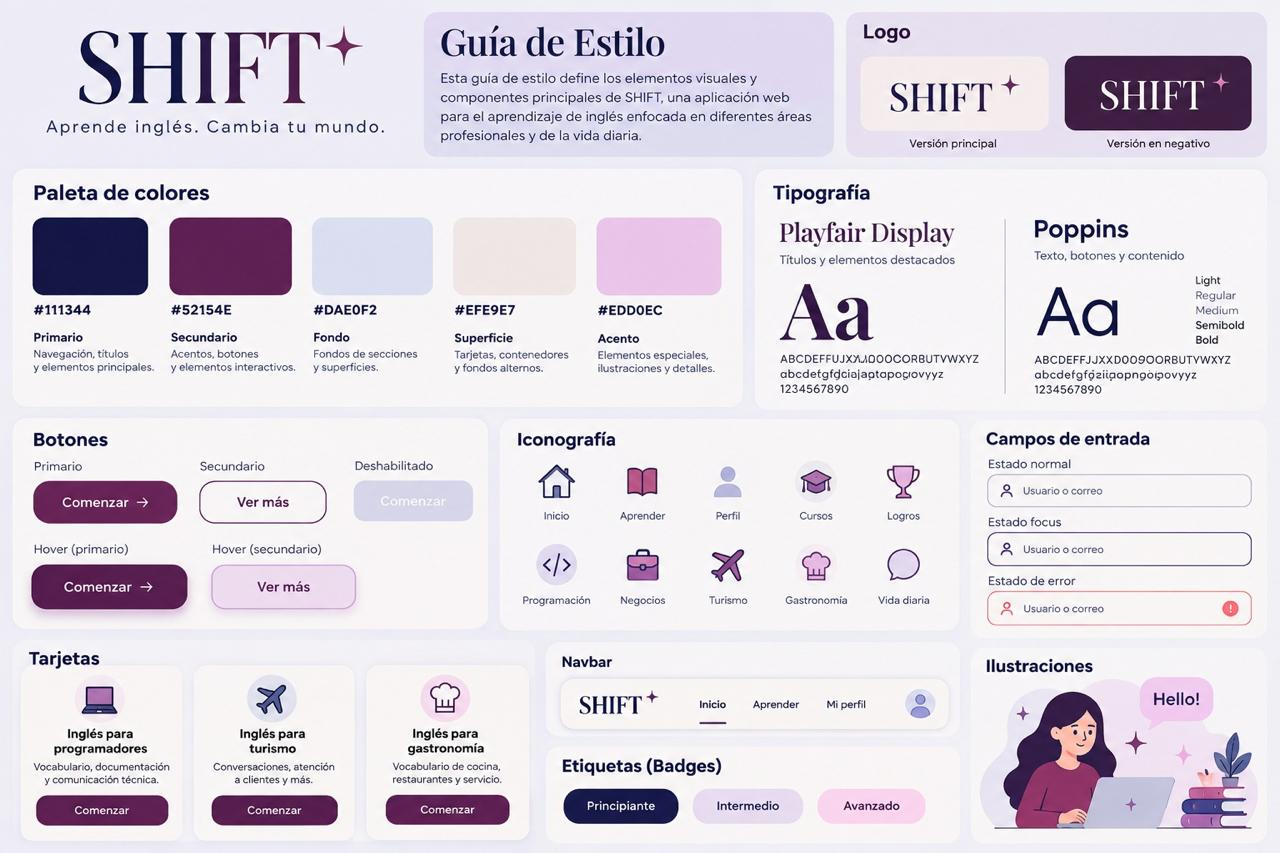
\includegraphics[width=\textwidth]{Guia de estilo.jpeg}
\caption{Guía de estilo }\label{fig:Guia de estilo}
\end{figure}

\section{Desarrollo y evidencias}
\subsection{Desarrollo del proyecto}
El desarrollo de la aplicación web SHIFTLY se realizó mediante un proceso
de trabajo colaborativo. Cada integrante del equipo recibió diferentes
interfaces y funcionalidades para desarrollar de acuerdo con la
distribución establecida mediante las actividades del proyecto.
\subsection{Desarrollo de interfaces}
A continuación se documentan las principales interfaces desarrolladas por
cada integrante del equipo, indicando la función de cada una y su
participación dentro del proyecto
\subsubsection{Registro de usuario}
\textbf{Descripción}
La interfaz de registro de usuario permite crear una cuenta en SHIFTLY
para acceder a la plataforma de aprendizaje de inglés. La pantalla
presenta un formulario de registro organizado en una tarjeta central, con
los elementos necesarios para introducir la información del usuario.
\textbf{Barra de navegación}
La parte superior de la interfaz contiene la identidad visual de SHIFTLY,
representada mediante el logotipo y el nombre de la aplicación. En la
parte derecha se encuentra la opción ``Iniciar Sesión'', destinada a los
usuarios que ya cuentan con una cuenta.
\textbf{Encabezado del formulario}
El formulario presenta el texto ``EMPIEZA HOY'' como encabezado y el título
``Crear Cuenta''. También incluye un mensaje introductorio que invita al
usuario a registrarse en SHIFTLY para comenzar su aprendizaje.
\textbf{Campos de registro}
La interfaz contiene tres campos de entrada para recopilar la información
necesaria para crear la cuenta:
\begin{itemize}
\item \textbf{Nombre Completo:} permite introducir el nombre del usuario.  
\item \textbf{Correo Electrónico:} permite introducir una dirección de
correo electrónico 
\item \textbf{Contraseña:} permite establecer una contraseña para la
cuenta. El campo indica como referencia un mínimo de 8 caracteres.
\end{itemize}
\textbf{Botón Crear Mi Cuenta}
El formulario incluye un botón denominado ``Crear Mi Cuenta'', destinado
a enviar la información introducida por el usuario para realizar el
registro en la plataforma
\textbf{Acceso para usuarios registrados}
Debajo del botón de registro se presenta el mensaje ``¿Ya tienes una
cuenta?'' junto con la opción ``Inicia sesión'', que permite dirigirse a
la pantalla de inicio de sesión para los usuarios que ya cuentan con una
cuenta
\textbf{Pie de página}
La parte inferior de la interfaz contiene un pie de página con el texto
``© 2026 Shiftly. Todos los derechos reservados.'', utilizado como
elemento informativo de la aplicación.
\textbf{Evidencia}
La siguiente captura muestra la interfaz de registro de usuario de
SHIFTLY
\begin{figure}[H]
\centering
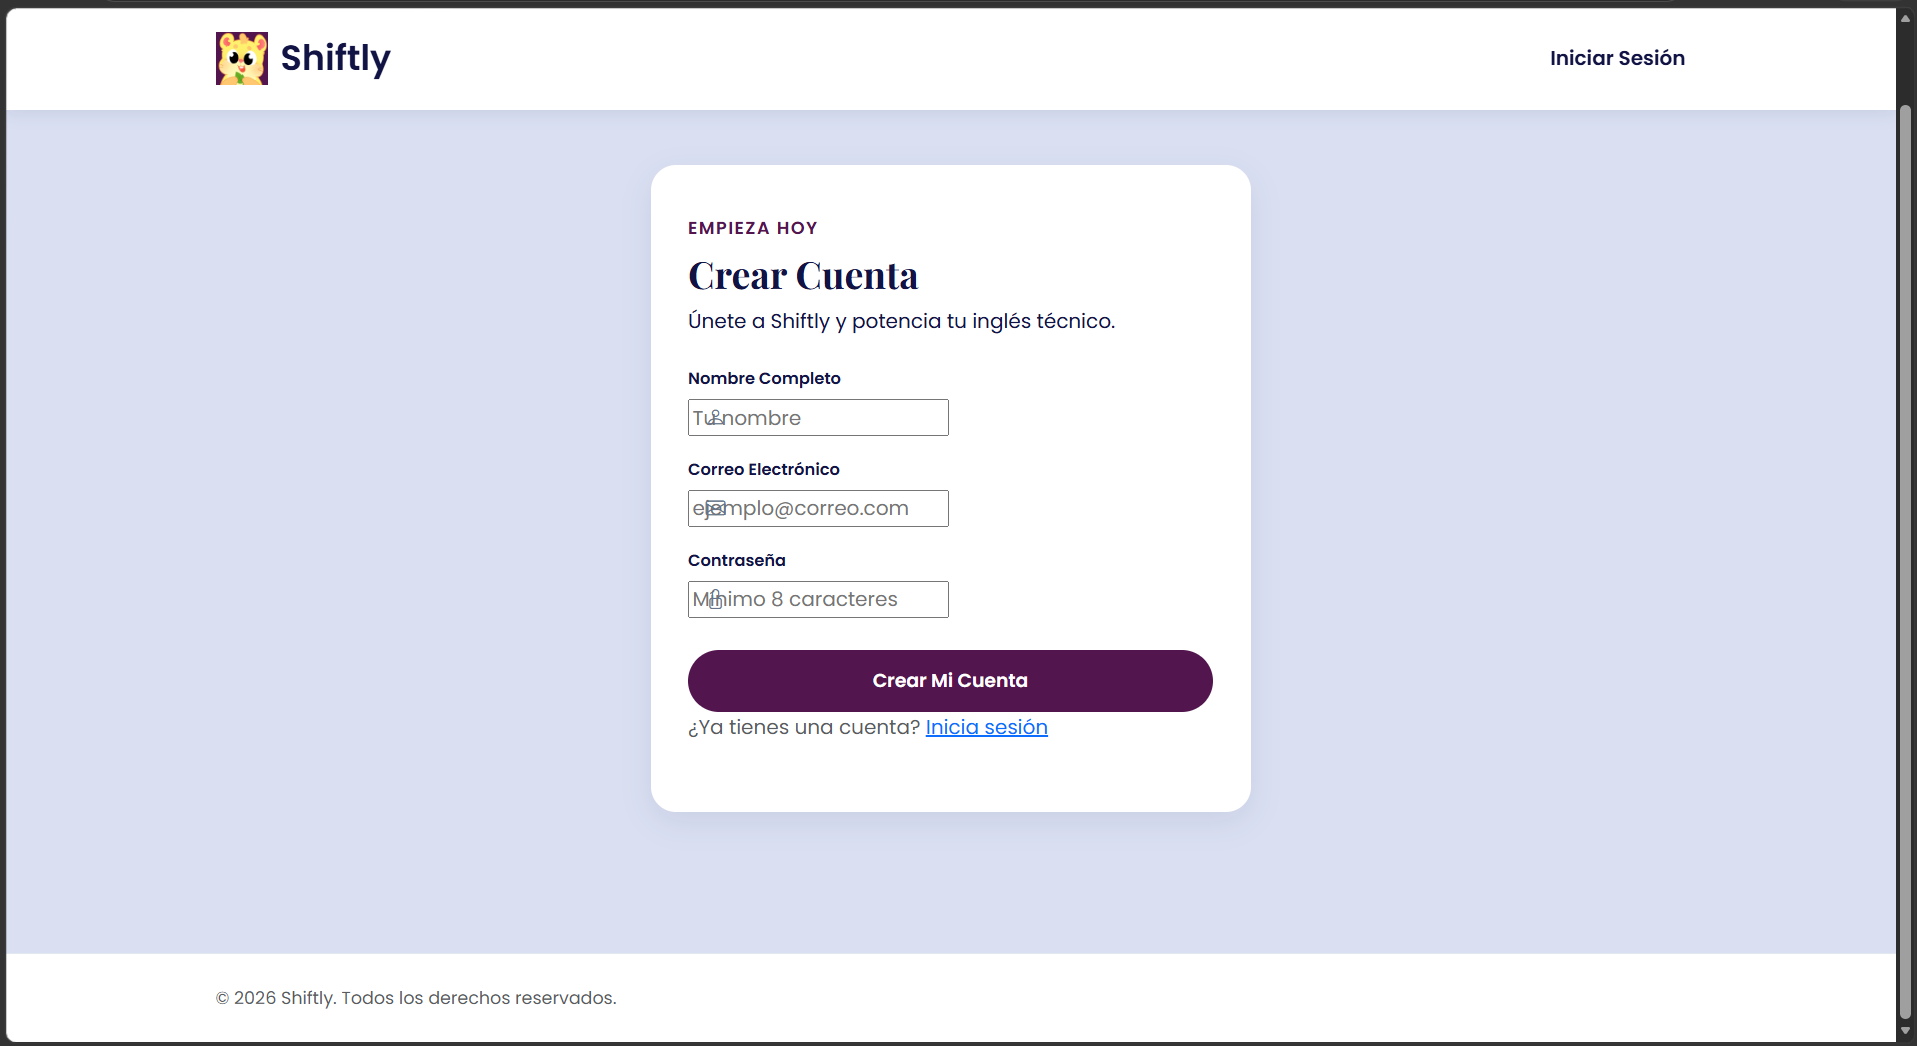
\includegraphics[width=\textwidth]{registro.png}
\caption{Interfaz de registro de usuario de SHIFTLY.}
\label{fig:registro}
\end{figure}
\subsubsection{Selección de áreas de aprendizaje}
La interfaz de selección de áreas de aprendizaje permite al usuario elegir
el área de inglés que desea aprender de acuerdo con sus intereses. Esta
sección presenta diferentes opciones mediante tarjetas interactivas y
proporciona un mecanismo para seleccionar una de ellas antes de continuar
con el proceso de aprendizaje\\
\textbf{Barra de navegación}\\
La parte superior de la interfaz contiene una barra de navegación que
incluye el nombre de SHIFTLY, el logotipo de la aplicación y las opciones
de navegación Inicio, Aprender, Mi perfil y Ayuda. Estos elementos forman
parte de la estructura general de navegación de la aplicación web\\
\textbf{Encabezado de la sección}\\
La sección presenta el título ``¿Qué inglés quieres aprender?'' junto con
un texto introductorio que explica al usuario que puede elegir un área de
aprendizaje para adaptar el contenido de acuerdo con sus intereses\\
\textbf{Áreas de aprendizaje}\\
La interfaz presenta cinco áreas de aprendizaje mediante tarjetas
individuales:
\begin{itemize}
\item \textbf{Programación:} presenta contenido de inglés enfocado en tecnología, desarrollo y mundo digital.
\item \textbf{Gastronomía:} presenta vocabulario, expresiones y situaciones relacionadas con el mundo culinario.
\item \textbf{Turismo:} presenta contenido relacionado con viajes, hoteles, atención al cliente y experiencias turísticas.
\item \textbf{Negocios:} presenta contenido orientado a ambientes profesionales, empresariales y comunicación laboral.
\item \textbf{Inglés cotidiano:} presenta expresiones y vocabulario relacionados con situaciones diarias de la vida real.
\end{itemize}
\textbf{Botones de selección}\\
Cada tarjeta contiene un botón denominado ``Seleccionar'' al presionar
este botón, el área correspondiente se identifica visualmente como la
opción seleccionada, cuando existe un área seleccionada, se permite continuar con el proceso de aprendizaje la integración con la siguiente interfaz se realizará posteriormente como parte del desarrollo colaborativo del proyecto.\\
\textbf{Botón Continuar}\\
La interfaz cuenta con un botón ``Continuar'' que permite avanzar al
siguiente paso del proceso, antes de continuar se verifica que el usuario
haya seleccionado un área de aprendizaje si el usuario intenta continuar sin seleccionar
un área, la aplicación muestra un mensaje solicitando realizar una selección, cuando existe un
área seleccionada, se permite continuar con el proceso de aprendizaje, la siguiente etapa del flujo corresponde al diagnóstico inicial, cuya integración con esta interfaz se realizará posteriormente como parte del desarrollo colaborativo del proyecto.
\begin{figure}[H]
\centering
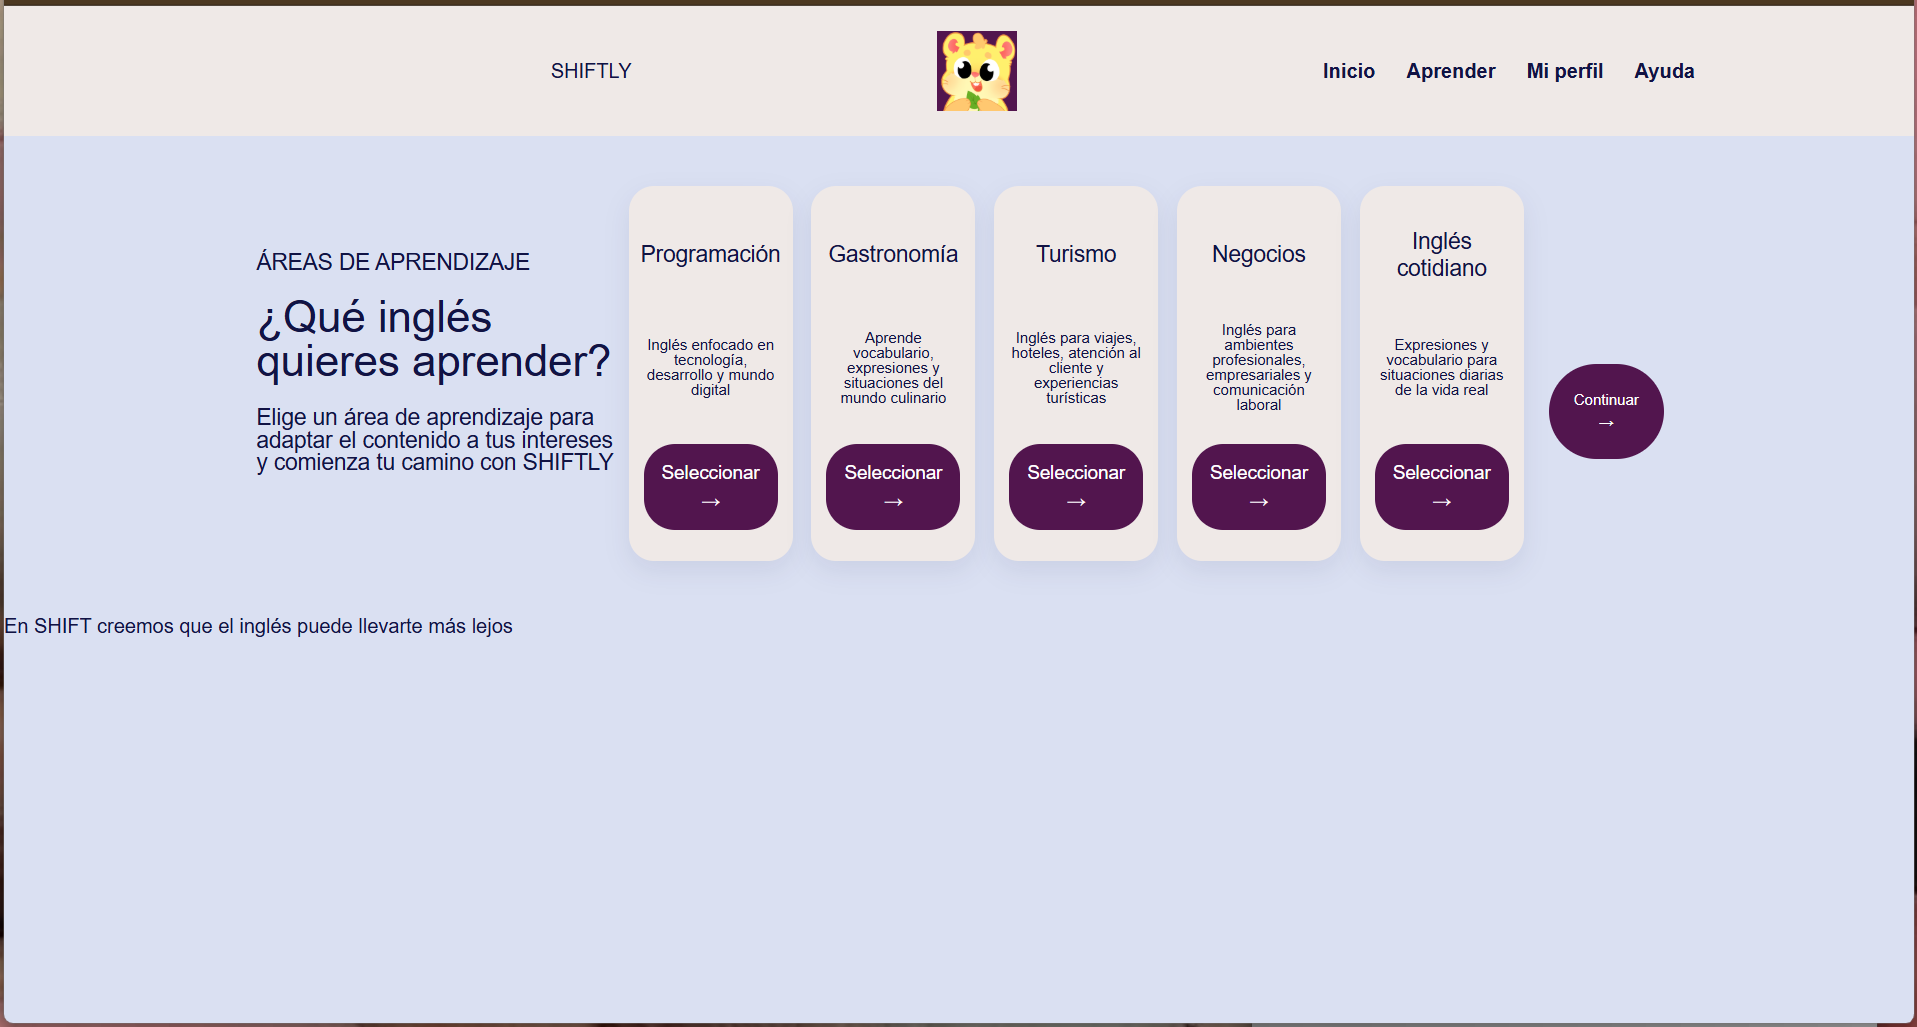
\includegraphics[width=\textwidth]{seleccion areas.png}
\caption{Interfaz de selección de áreas de aprendizaje en SHIFTLY}
\label{fig:seleccion areas}
\end{figure}
\subsubsection{Diagnóstico inicial}
\textbf{Descripción}
La interfaz de diagnóstico inicial permite al usuario realizar una
evaluación para conocer su nivel actual de inglés. La pantalla presenta
una serie de preguntas con diferentes opciones de respuesta y muestra el
avance del usuario durante el diagnóstico.
\textbf{Barra de navegación}
La parte superior de la interfaz contiene la barra de navegación de
SHIFTLY. En ella se muestra el logotipo y nombre de la aplicación, así
como las opciones ``Inicio'', ``Aprender'', ``Mi perfil'' y ``Ayuda''.
\textbf{Encabezado del diagnóstico}
La sección principal presenta la etiqueta ``TEST DE DIAGNÓSTICO'' y el
título ``Descubre tu nivel de inglés''. También incluye un texto
introductorio que explica al usuario que debe responder las preguntas
para conocer su nivel actual y recibir recomendaciones de aprendizaje.
\textbf{Indicador de progreso}
La interfaz incorpora una sección denominada ``Progreso'' que permite
visualizar el avance del usuario dentro del diagnóstico. En la captura se
muestra el indicador ``1 de 5'', acompañado de una barra de progreso que
representa el avance de la evaluación.
\textbf{Pregunta de diagnóstico}
La pantalla presenta la ``Pregunta 1'' dentro de una tarjeta de
contenido. La pregunta mostrada es ``Choose the correct option:'' y se
presentan diferentes alternativas para responderla.
\begin{itemize}
\item \textbf{She are a student.}
\item \textbf{She is a student.}
\item \textbf{She am a student.}
\item \textbf{She be a student.}
\end{itemize}
Las opciones permiten al usuario identificar la respuesta que considera
correcta para continuar con el diagnóstico.
\textbf{Pie de página}
En la parte inferior de la interfaz se presenta el mensaje ``En Shiftly
creemos que el inglés puede llevarte más lejos'', utilizado como elemento
informativo de la aplicación.
\textbf{Evidencia}
La siguiente captura muestra la interfaz del diagnóstico inicial de
SHIFTLY
\begin{figure}[H]
\centering
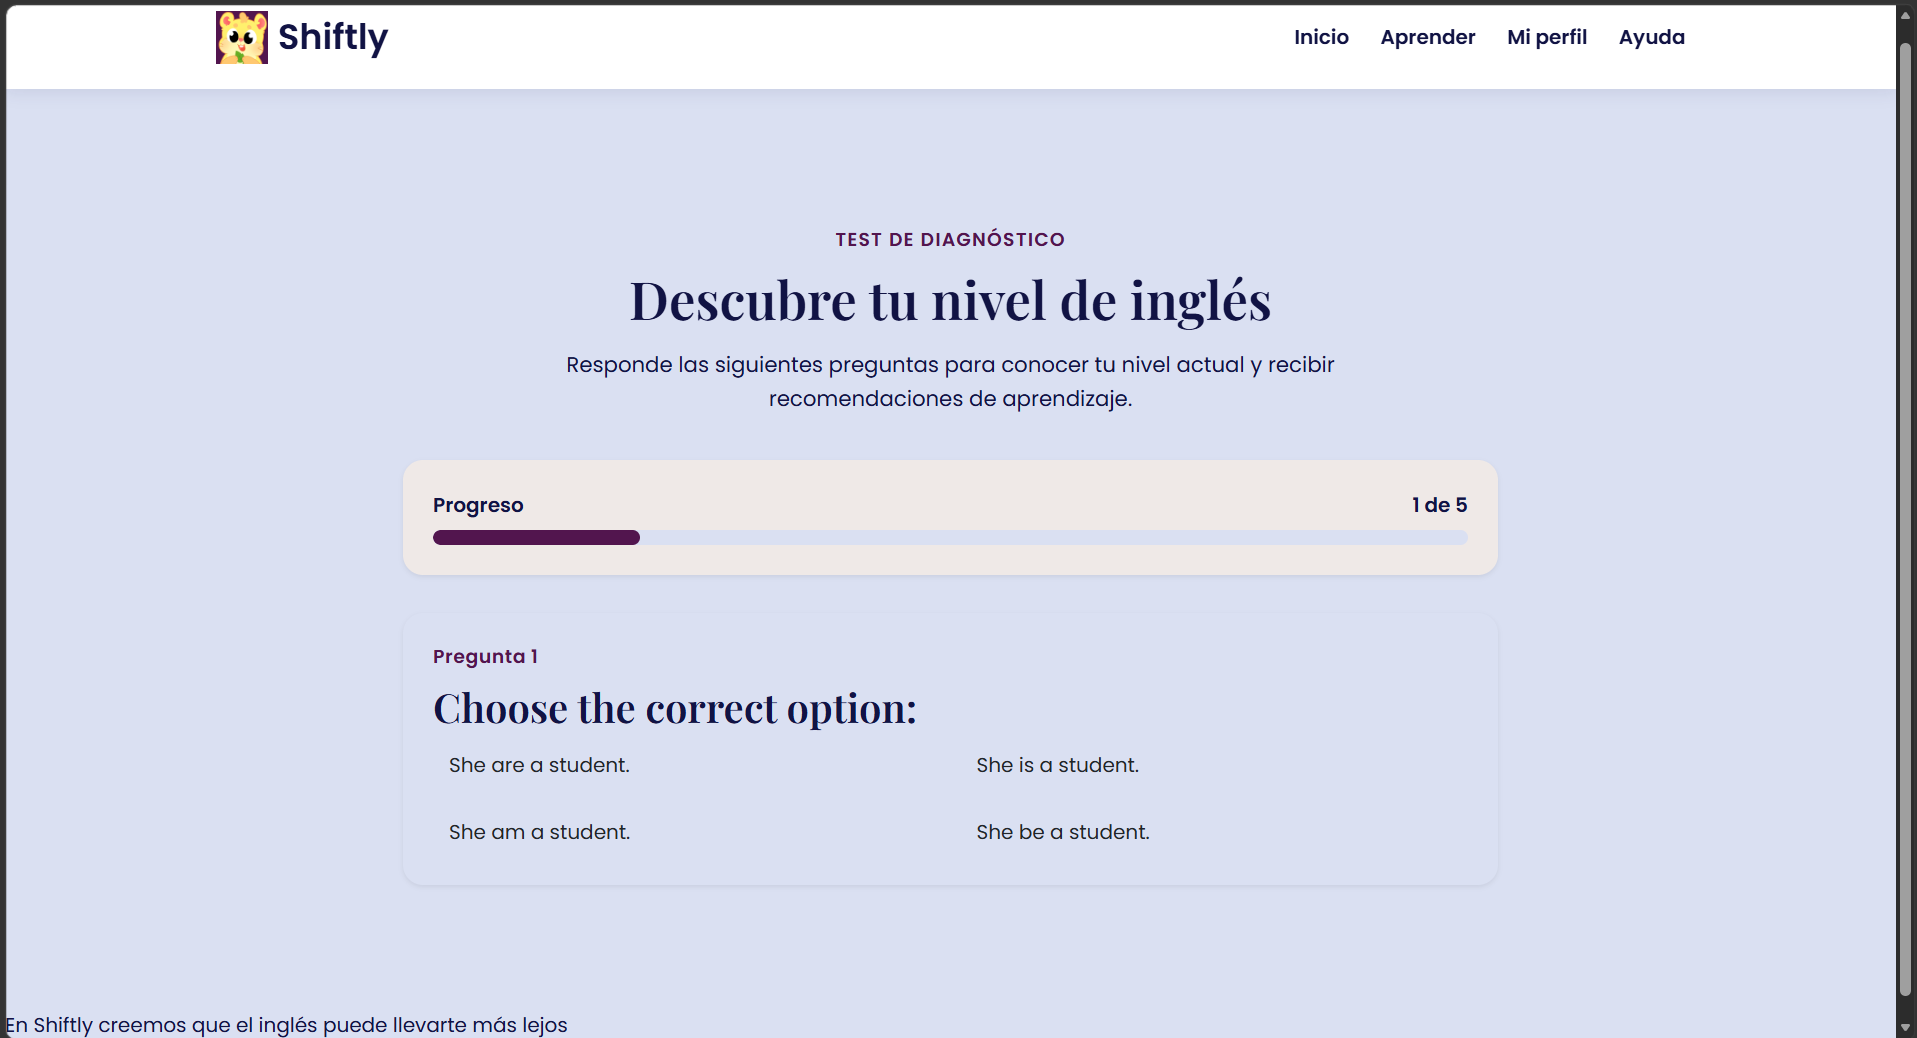
\includegraphics[width=\textwidth]{diagnostico.png}
\caption{Interfaz de diagnóstico inicial de SHIFTLY.}
\label{fig:diagnostico}
\end{figure}
\subsubsection{Vaneza Lugo Ramírez}
\textbf{Tarjetas de vocabulario}
Esta interfaz corresponde a las tarjetas de aprendizaje utilizadas para
presentar vocabulario en inglés, incluyendo información relacionada con
las palabras y su aprendizaje.
\textbf{Evidencia:}
\textit{En este apartado se colocará la captura de las tarjetas de
vocabulario.}
\vspace{0.5cm}
\textbf{Biblioteca y repaso}
Esta interfaz corresponde a la sección destinada al repaso de contenidos
y vocabulario previamente estudiado por el usuario.
\textbf{Evidencia:}
\textit{En este apartado se colocará la captura de la biblioteca y sección
de repaso.}
\subsubsection{Brian Jael Juárez Rodríguez}
\textbf{Ejercicios interactivos}
Esta interfaz corresponde a las actividades interactivas utilizadas para
que el usuario practique los contenidos de aprendizaje mediante diferentes
ejercicios.
\textbf{Evidencia:}
\textit{En este apartado se colocará la captura de los ejercicios
interactivos.}
\subsubsection{Julio}
\textbf{Mapa de lecciones}
Esta interfaz representa la ruta de aprendizaje del usuario mediante un
mapa o estructura de lecciones.
\textbf{Evidencia:}
\textit{En este apartado se colocará la captura del mapa de lecciones.}
\vspace{0.5cm}
\textbf{Siguiente lección recomendada}
Esta interfaz corresponde a la sección encargada de mostrar al usuario una
recomendación de la siguiente lección dentro de su proceso de aprendizaje.
\textbf{Evidencia:}
\textit{En este apartado se colocará la captura de la siguiente lección
recomendada.}
\subsection{Control de versiones}
El proyecto utiliza Git y GitHub para administrar el código fuente y
mantener un registro de los cambios realizados durante el desarrollo.
El trabajo se organizó mediante ramas para desarrollar las diferentes
funcionalidades de manera independiente antes de integrarlas al proyecto
principal.
\textbf{Evidencia:}
\textit{En este apartado se colocará la captura del repositorio y las ramas
utilizadas.}
\subsection{Commits}
Durante el desarrollo se realizaron commits descriptivos para registrar
los avances realizados en la aplicación web.
En el caso de la interfaz de selección de áreas de aprendizaje se
realizaron diferentes commits relacionados con la estructura de la
pantalla, las áreas de aprendizaje, la selección de áreas y la validación
del botón de continuar.
\textbf{Evidencia:}
\textit{En este apartado se colocará la captura del historial de commits.}
\subsection{Pull Request}
Después de completar el desarrollo de la funcionalidad correspondiente, se
creó un Pull Request para solicitar la integración de los cambios a la
rama principal del proyecto.
\textbf{Evidencia:}
\textit{En este apartado se colocará la captura del Pull Request.}
\subsection{Tablero Kanban}
El desarrollo del proyecto se organizó mediante un tablero Kanban para
dar seguimiento al avance de las actividades asignadas a los integrantes
del equipo.
\textbf{Evidencia:}
\textit{En este apartado se colocará la captura del tablero Kanban.}
\subsection{Pruebas responsive}
La aplicación web SHIFTLY se diseñó considerando diferentes tamaños de
pantalla. Para comprobar su adaptación se realizarán capturas de la
aplicación en computadora y en dispositivos móviles.
\textbf{Evidencia:}
\textit{En este apartado se colocarán las capturas de la aplicación en
computadora y teléfono móvil.}

\clearpage

\section{Conclusiones}
\input{Conclusion.tex}


%-------------------------------------------------------------------------------
% REFERENCES
%-------------------------------------------------------------------------------
\newpage
\section*{References}

%[2]John W. Eaton, David Bateman, Sren Hauberg, Rik Wehbring (2015). GNU
%Octave version 4.0.0 manual: a high-level interactive language for numer-
%ical computations. Available: http://www.gnu.org/software/octave/doc/
%interpreter/. 
}
\end{document}

%-------------------------------------------------------------------------------
% SNIPPETS
%-------------------------------------------------------------------------------

%\begin{figure}[!ht]
%	\centering
%	\includegraphics[width=0.8\textwidth]{file_name}
%	\caption{}
%	\centering
%	\label{label:file_name}
%\end{figure}

%\begin{figure}[!ht]
%	\centering
%	\includegraphics[width=0.8\textwidth]{graph}
%	\caption{Blood pressure ranges and associated level of hypertension (American Heart Association, 2013).}
%	\centering
%	\label{label:graph}
%\end{figure}

%\begin{wrapfigure}{r}{0.30\textwidth}
%	\vspace{-40pt}
%	\begin{center}
%		\includegraphics[width=0.29\textwidth]{file_name}
%	\end{center}
%	\vspace{-20pt}
%	\caption{}
%	\label{label:file_name}
%\end{wrapfigure}

%\begin{wrapfigure}{r}{0.45\textwidth}
%	\begin{center}
%		\includegraphics[width=0.29\textwidth]{manometer}
%	\end{center}
%	\caption{Aneroid sphygmomanometer with stethoscope (Medicalexpo, 2012).}
%	\label{label:manometer}
%\end{wrapfigure}

%\begin{table}[!ht]\footnotesize
%	\centering
%	\begin{tabular}{cccccc}
%	\toprule
%	\multicolumn{2}{c} {Pearson's correlation test} & \multicolumn{4}{c} {Independent t-test} \\
%	\midrule	
%	\multicolumn{2}{c} {Gender} & \multicolumn{2}{c} {Activity level} & \multicolumn{2}{c} {Gender} \\
%	\midrule
%	Males & Females & 1st level & 6th level & Males & Females \\
%	\midrule
%	\multicolumn{2}{c} {BMI vs. SP} & \multicolumn{2}{c} {Systolic pressure} & \multicolumn{2}{c} {Systolic Pressure} \\
%	\multicolumn{2}{c} {BMI vs. DP} & \multicolumn{2}{c} {Diastolic pressure} & \multicolumn{2}{c} {Diastolic pressure} \\
%	\multicolumn{2}{c} {BMI vs. MAP} & \multicolumn{2}{c} {MAP} & \multicolumn{2}{c} {MAP} \\
%	\multicolumn{2}{c} {W:H ratio vs. SP} & \multicolumn{2}{c} {BMI} & \multicolumn{2}{c} {BMI} \\
%	\multicolumn{2}{c} {W:H ratio vs. DP} & \multicolumn{2}{c} {W:H ratio} & \multicolumn{2}{c} {W:H ratio} \\
%	\multicolumn{2}{c} {W:H ratio vs. MAP} & \multicolumn{2}{c} {\% Body fat} & \multicolumn{2}{c} {\% Body fat} \\
%	\multicolumn{2}{c} {} & \multicolumn{2}{c} {Height} & \multicolumn{2}{c} {Height} \\
%	\multicolumn{2}{c} {} & \multicolumn{2}{c} {Weight} & \multicolumn{2}{c} {Weight} \\
%	\multicolumn{2}{c} {} & \multicolumn{2}{c} {Heart rate} & \multicolumn{2}{c} {Heart rate} \\
%	\bottomrule
%	\end{tabular}
%	\caption{Parameters that were analysed and related statistical test performed for current study. BMI - body mass index; SP - systolic pressure; DP - diastolic pressure; MAP - mean arterial pressure; W:H ratio - waist to hip ratio.}
%	\label{label:tests}
%\end{table}%\documentclass{article}
%\usepackage[utf8]{inputenc}

%\title{Weekly Report template}
%\author{gandhalijuvekar }
%\date{January 2019}

%\begin{document}

%\maketitle

%\section{Introduction}

%\end{document}
